\documentclass{beamer}
\usepackage[latin9]{inputenc}
\usepackage{xcolor}
\usepackage{graphics, graphicx}
\usepackage{tikz, tkz-graph}
\usepackage{pgf, pgfplots}
\usepackage{graphviz, tkz-berge}
\usepackage{graphics, graphicx}
\usepackage{pstricks, pst-node, pst-tree}
\usepackage{float}
\usepackage{amstext}
\usepackage{amsmath}
\usepackage{amsfonts}
\usepackage{mathtools}
\usepackage{minted}
\usepackage[ruled, boxed]{algorithm2e}
\usepackage{multicol, multirow, rotating} %Paquets de taules
\usepackage{float} %Imatges m�ltiples
\usepackage{verbatim}
\usepackage[style=english]{csquotes}
\usepackage{cancel}
\usepackage[position=top]{subfig}
\usepackage{rotating}
\usepackage{etoolbox}
\usepackage{parskip}
\usepackage[bottom]{footmisc}
\usepackage[toc,page]{appendix}
\usepackage{caption}
\captionsetup[figure]{labelformat=empty}


\usetikzlibrary{arrows, petri, topaths}
\usetikzlibrary{shapes}
\usetikzlibrary{arrows.meta}
\usetikzlibrary{positioning,automata}

\usetheme{Warsaw}
\mode<presentation>{\usetheme{Warsaw}}
\setbeamertemplate{caption}{\raggedright\insertcaption\par}

\graphicspath{ {altres/graphics/} }


\title{Els grafs: xarxes, camins i connexions}
 
\subtitle{De la matem�tica discreta a la realitat}
 
\author{Aniol Garcia i Serrano}
 

\date[Presentaci� TDR] % (optional)
{Presentaci� del treball, Gener 2017}



\begin{document}

\setbeamertemplate{caption}{\raggedright\insertcaption\par}
%\begin{frame}{Overview}
%\tableofcontents
%\end{frame}

\frame{\titlepage}

\section{Introducci�}
\subsection{El meu primer graf}
\begin{frame}
\frametitle{El meu primer graf}
	\begin{figure}[H]
		\includegraphics[scale=0.3]{graf1}
	\end{figure}
\end{frame}

\subsection{El primer graf}
\begin{frame}
\frametitle{El primer graf}
\begin{columns}
 
\column{0.5\textwidth}
\begin{figure}[H]
\centering
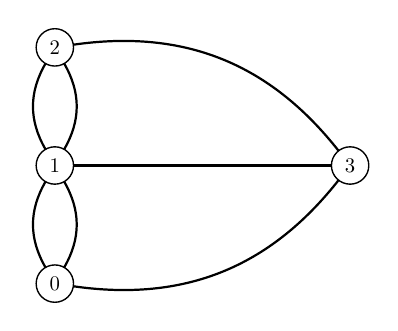
\begin{tikzpicture}[scale=0.75,transform shape]
  \Vertex[x=0,y=0]0
  \Vertex[x=0,y=2]1
  \Vertex[x=0,y=4]2
  \Vertex[x=5,y=2]3
  \tikzstyle{LabelStyle}=[fill=white,sloped]
  \Edge(1)(3)
  \tikzstyle{EdgeStyle}=[bend left]
  \Edge(0)(1)
  \Edge(1)(2)
  \Edge(2)(3)
  \tikzstyle{EdgeStyle}=[bend right]
  \Edge(0)(1)
  \Edge(1)(2)
  \Edge(0)(3)
\end{tikzpicture}
\end{figure}

\pause

\column{0.5\textwidth}
\includegraphics[scale=0.5]{Konigsberg_bridges}

\end{columns}
\end{frame}

\subsection{Breu hist�ria}
\begin{frame}
\frametitle{Breu hist�ria}
\begin{columns}
 
\column{0.5\textwidth}
	\begin{figure}[H]
		\includegraphics[scale=0.21405]{Euler}
		\caption{Leonhard Euler}
	\end{figure}
\column{0.5\textwidth}
	\begin{figure}[H]
		\includegraphics[scale=0.4]{Leibniz}
		\caption{Gottfried W. Leibniz}
	\end{figure}
\end{columns}
\end{frame}

\frame{\titlepage}


\section{Organitzaci�}
%\begin{frame}
%\tableofcontents
%No hi ha d'haver aquest �ndex, sin� el del treball (simplificat, evidentment)
%\end{frame}
\subsection{Objectius}
\begin{frame}
\frametitle{Objectius}
\begin{itemize}
\item Con�ixer la teoria de grafs
\item Estudiar i implementar algorismes
\item Mostrar-ne algunes de les aplicacions
\end{itemize}
\end{frame}


\subsection{Tipus de grafs}
\begin{frame}
\frametitle{Tipus de grafs}

\begin{figure}[H]
				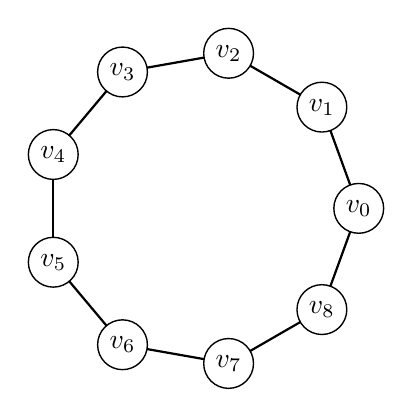
\begin{tikzpicture}	
		\grCycle[RA=2, prefix=v, Math=true]{9}
		\end{tikzpicture}
		\caption{Cicle}	
\end{figure}
\end{frame}

\begin{frame}
\begin{figure}[H]
		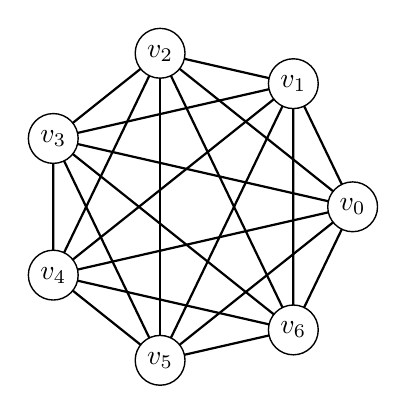
\begin{tikzpicture}	
			\grComplete[RA=2, prefix=v, Math=true]{7}
		\end{tikzpicture}
		\caption{Complet}	
\end{figure}
\end{frame}

\begin{frame}
\begin{figure}[H]
		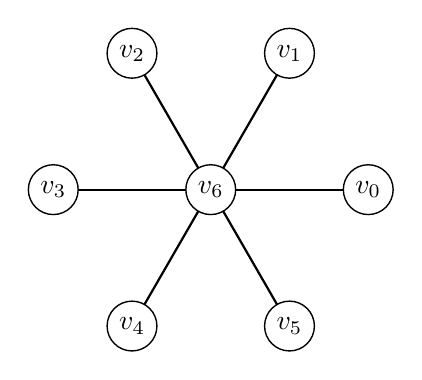
\begin{tikzpicture}	
		\grStar[RA=2, prefix=v, Math=true]{7}	
		\end{tikzpicture}
		\caption{Estrella}	
\end{figure}
\end{frame}

\begin{frame}
\begin{figure}[H]
		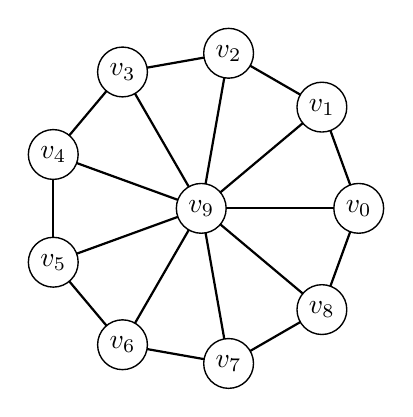
\begin{tikzpicture}	
		\grWheel[RA=2, prefix=v, Math=true]{10}	
		\end{tikzpicture}
		\caption{Roda}	
\end{figure}
\end{frame}

\begin{frame}
\begin{figure}[H]
		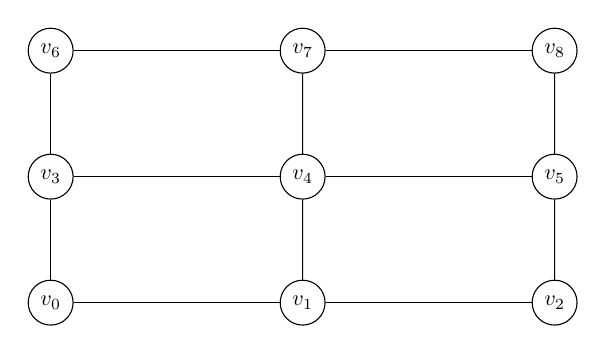
\begin{tikzpicture}[round/.style={circle, draw=black, thin, minimum 			size=.5mm}, transform shape, scale=0.80]
		\node[round] (a) at (0,0){$v_{0}$};
		\node[round] (b) at (4,0){$v_{1}$};
		\node[round] (c) at (8,0){$v_{2}$};
		\node[round] (d) at (0,2){$v_{3}$};
		\node[round] (e) at (4,2){$v_{4}$};
		\node[round] (f) at (8,2){$v_{5}$};
		\node[round] (g) at (0,4){$v_{6}$};
		\node[round] (h) at (4,4){$v_{7}$};
		\node[round] (i) at (8,4){$v_{8}$};
		\draw (a) edge (b);
		\draw (a) edge (d);
		\draw (b) edge (c);
		\draw (b) edge (e);
		\draw (c) edge (f);
		\draw (d) edge (e);
		\draw (d) edge (g);
		\draw (e) edge (h);
		\draw (e) edge (f);
		\draw (f) edge (i);
		\draw (h) edge (i);
		\draw (h) edge (g);
		\end{tikzpicture}
		\caption{Xarxa}	
\end{figure}
\end{frame}

\begin{frame}
\begin{columns}
\column{0.5\textwidth}
\begin{figure}[H]
		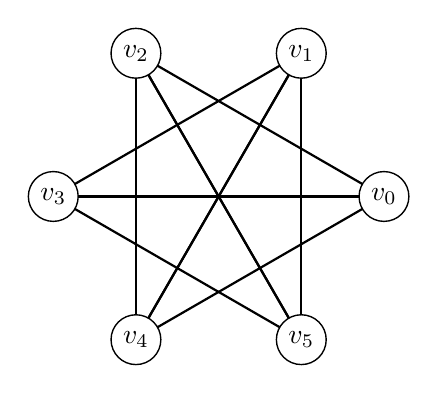
\begin{tikzpicture}[scale=0.7]	
		\grCirculant[RA=3, prefix=v,Math=true]{6}{2,3}
		\end{tikzpicture}	
		\caption{Graf G}
\end{figure}
\column{0.5\textwidth}
\begin{figure}[H]
		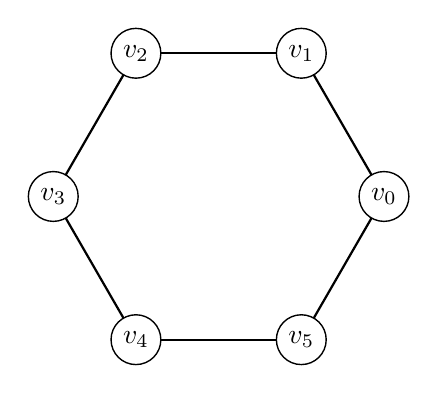
\begin{tikzpicture}[scale=0.7]	
				\grCirculant[RA=3, prefix=v,Math=true]{6}{1}
		\end{tikzpicture}
		\caption{Complementari de G}	
\end{figure}
\end{columns}
\end{frame}

\begin{frame}
\begin{figure}[H]
		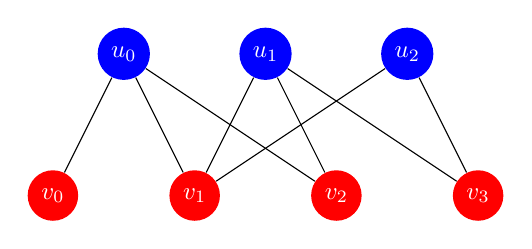
\begin{tikzpicture}[v/.style={circle, fill=red, text=white, thin, minimum size=.5mm}, u/.style={circle, fill=blue, text=white, thin, minimum size=.5mm}, transform shape, scale=0.90]
		\node[v] (a) at (0,0){$v_{0}$};
		\node[v] (b) at (2,0){$v_{1}$};
		\node[v] (c) at (4,0){$v_{2}$};
		\node[v] (d) at (6,0){$v_{3}$};
		\node[u] (e) at (1,2){$u_{0}$};
		\node[u] (f) at (3,2){$u_{1}$};
		\node[u] (g) at (5,2){$u_{2}$};
		\draw (a) edge (e);
		\draw (b) edge (e);
		\draw (b) edge (f);
		\draw (b) edge (g);
		\draw (c) edge (e);
		\draw (c) edge (f);
		\draw (d) edge (f);
		\draw (d) edge (g);
		\end{tikzpicture}
		\caption{Bipartit}	
\end{figure}
\end{frame}

\begin{frame}
\begin{figure}[H]
		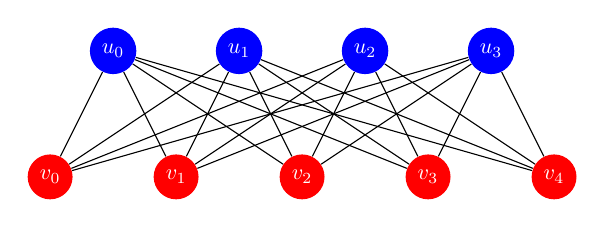
\begin{tikzpicture}[v/.style={circle, fill=red, text=white, thin, minimum size=.5mm}, u/.style={circle, fill=blue, text=white, thin, minimum size=.5mm}, transform shape, scale=0.80]
		\node[v] (a) at (0,0){$v_{0}$};
		\node[v] (b) at (2,0){$v_{1}$};
		\node[v] (c) at (4,0){$v_{2}$};
		\node[v] (d) at (6,0){$v_{3}$};
		\node[v] (h) at (8,0){$v_{4}$};
		\node[u] (e) at (1,2){$u_{0}$};
		\node[u] (f) at (3,2){$u_{1}$};
		\node[u] (g) at (5,2){$u_{2}$};
		\node[u] (i) at (7,2){$u_{3}$};
		\draw (a) edge (e);
		\draw (a) edge (f);
		\draw (a) edge (g);
		\draw (a) edge (i);
		\draw (b) edge (e);
		\draw (b) edge (f);
		\draw (b) edge (g);
		\draw (b) edge (i);
		\draw (c) edge (e);
		\draw (c) edge (f);
		\draw (c) edge (g);
		\draw (c) edge (i);
		\draw (d) edge (e);
		\draw (d) edge (f);
		\draw (d) edge (g);
		\draw (d) edge (i);
		\draw (h) edge (e);
		\draw (h) edge (f);
		\draw (h) edge (g);
		\draw (h) edge (i);
		\end{tikzpicture}
		\caption{Bipartit complet}	
\end{figure}
\end{frame}

\begin{frame}
\begin{figure}[H]
		\begin{tikzpicture}[round/.style={circle, draw=black, thin, minimum 			size=.5mm}, transform shape, scale=0.80]
		\node[round] (a) at (0,0){$v_{0}$};
		\node[round] (b) at (4,0){$v_{1}$};
		\node[round] (c) at (8,0){$v_{2}$};
		\node[round] (d) at (0,2){$v_{3}$};
		\node[round] (d) at (4,2){$v_{4}$};
		\node[round] (d) at (8,2){$v_{5}$};
		\end{tikzpicture}
		\caption{Buit}	
\end{figure}
\end{frame}

\begin{frame}
\begin{figure}[H]
		\begin{tikzpicture}	

		\end{tikzpicture}
		\caption{Nul}	
\end{figure}
\end{frame}


\begin{frame}
\begin{figure}[H]
		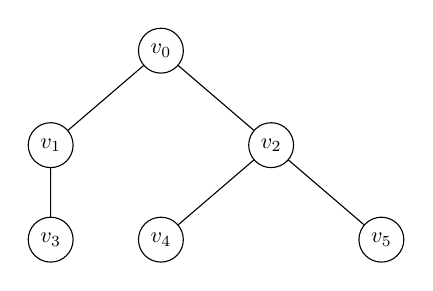
\begin{tikzpicture}[round/.style={circle, draw=black, thin, minimum 			size=.5mm}, transform shape, scale=0.80]
			\tikzstyle{level 1}=[level distance=15mm,sibling distance=35mm]
			\node(0)[round]{$v_{0}$}
				child{node[round]{$v_{1}$}
					child{node[round]{$v_{3}$}}}
				child{node[round]{$v_{2}$}
					child{node[round]{$v_{4}$}}
					child{node[round]{$v_{5}$}}
			};
		\end{tikzpicture}
		\caption{Arbre}	
\end{figure}
\end{frame}


\begin{frame}
\begin{figure}[H]
		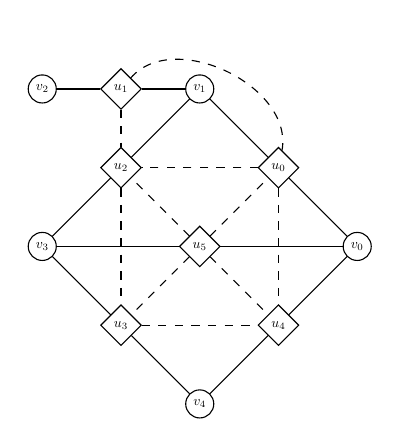
\begin{tikzpicture}[round/.style={circle, draw=black, thin, minimum size=.5mm}, transform shape, scale=0.5]
			\node[round] (a) at (8,4){$v_{0}$};
			\node[round] (b) at (4,8){$v_{1}$};
			\node[round] (c) at (0,8){$v_{2}$};
			\node[round] (d) at (0,4){$v_{3}$};
			\node[round] (e) at (4,0){$v_{4}$};
			\node[draw, diamond] (f) at (6,6){$u_{0}$};
			\node[draw, diamond] (g) at (2,8){$u_{1}$};
			\node[draw, diamond] (h) at (2,6){$u_{2}$};
			\node[draw, diamond] (i) at (2,2){$u_{3}$};
			\node[draw, diamond] (j) at (6,2){$u_{4}$};
			\node[draw, diamond] (k) at (4,4){$u_{5}$};
			\draw (a) edge (f);
			\draw (a) edge (j);
			\draw (a) edge (k);
			\draw (f) edge (b);
			\draw (j) edge (e);
			\draw (k) edge (d);
			\draw (b) edge (g);
			\draw (g) edge (c);
			\draw (b) edge (h);
			\draw (h) edge (d);
			\draw (d) edge (i);
			\draw (i) edge (e);
			
			\draw (f) edge[dashed] (h);
			\draw (k) edge[dashed] (f);
			\draw (k) edge[dashed] (j);
			\draw (k) edge[dashed] (i);
			\draw (k) edge[dashed] (h);
			\draw (f) edge[dashed] (h);
			\draw (i) edge[dashed] (j);
			\draw (g) edge[dashed] (h);
			\draw (f) edge[dashed] (j);
			\draw (h) edge[dashed] (i);
			\draw (g) edge[dashed, bend left=75] (f);
			
		\end{tikzpicture}
		\caption{Graf Lineal}	
\end{figure}

\end{frame}

\begin{frame}
\frametitle{Propietats i demostracions}
A tall d'exemple:

\begin{figure}[H]
		\includegraphics[scale=0.2]{propietat}
\end{figure}
\end{frame}

\begin{frame}
\frametitle{Altres classificacions}
\begin{columns}
\column{0.5\textwidth}
	\begin{figure}[H]
		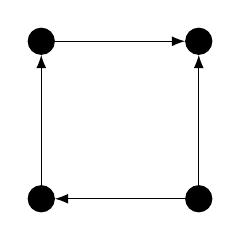
\begin{tikzpicture}[round/.style={circle, draw=black, fill=black, thin, minimum size=1mm}, transform shape]
			\node[round] (a) at (0,0){};
			\node[round] (b) at (0,2) {};
			\node[round] (c) at (2,0) {};
			\node[round] (d) at (2,2) {};
			\draw (a) edge[->, -Latex] (b);
			\draw (c) edge[->, -Latex] (a);
			\draw (b) edge[->, -Latex] (d);
			\draw (c) edge[->, -Latex] (d);
		\end{tikzpicture}
		\caption{Graf dirigit}
	\end{figure}
\column{0.5\textwidth}
\begin{figure}[H]
		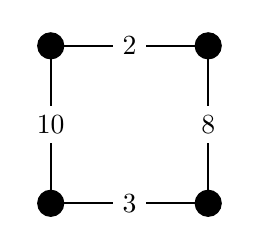
\begin{tikzpicture}[round/.style={circle, draw=black, fill=black, thin, minimum size=1mm}, transform shape]
			\node[round] (a) at (0,0){};
			\node[round] (b) at (0,2) {};
			\node[round] (c) at (2,0) {};
			\node[round] (d) at (2,2) {};
			\Edge[label=$10$](a)(b)
			\Edge[label=$3$](c)(a)
			\Edge[label=$2$](b)(d)
			\Edge[label=$8$](c)(d)
		\end{tikzpicture}
		\caption{Graf ponderat}
	\end{figure}

\end{columns}
\end{frame}

\subsection{Algorismes}
\begin{frame}
\frametitle{Algorismes}
\begin{itemize}
\item Camins
	\begin{itemize}
	\item Euler
	\item Hamilton
	\item Dijkstra
	\item Bellman-Ford
	\item Floyd-Warshall
	\end{itemize}
\item MST
	\begin{itemize}
	\item Kruskal
	\item Prim
	\end{itemize}
\item Exploraci�
	\begin{itemize}
	\item DFS
	\item BFS
	\end{itemize}
\item Coloraci�
	\begin{itemize}
	\item DFS
	\item El meu propi algorisme
	\end{itemize}
\end{itemize}
\end{frame}

\section{Aplicacions}
\subsection{Metro}

\begin{frame}
\frametitle{Plantejament}
\begin{figure}[H]
		\includegraphics[scale=0.2]{metro}
\end{figure}
\end{frame}

\begin{frame}
\frametitle{Organitzaci�}
\begin{figure}[H]
		\includegraphics[scale=0.25]{metro4}
\end{figure}
\end{frame}

\begin{frame}[fragile]
\begin{minted}[frame=lines, breaklines=true, baselinestretch=1, fontsize=\fontsize{4}{6}]{python}
def metro(Adj, inici, final, k): #on k �s el temps de parada acada estaci�
    recorregut=[]
    
    print "Punt inicial:", inici.decode("ISO-8859-15")
    
    print "Punt final:", final.decode("ISO-8859-15")

    dist, tree = OrderedDijkstra(Adj, inici, k)

    i = final    
    while tree[i] != inici:
        recorregut.append(tree[i])
        i = tree[i]
    
    recorregut.append(inici)        
    recorregut.reverse()

    total= dist[final]-k

    print "Temps amb estacions del recorregut:", dist[final], "Temps real:", total    
    
    if total < 60:
        print "Temps total del recorregut:",int(total), "segons"        
    else:
        minuts = total/60
        segons = (total%60)
        print "Temps total del recorregut:", int(minuts),"minuts i", int(segons), "segons"

    print "Recorregut:",   
    print "[",
    for i in range(0,len(recorregut)):
        print recorregut[i].decode("ISO-8859-15")+",",

    print final.decode("ISO-8859-15"),"]" 
\end{minted}
\end{frame}

\begin{frame}[fragile]
\begin{minted}[frame=lines, breaklines=true]{python}
def OrderedDijkstra(Adj, s, k):
    Q = dict.fromkeys(Adj.keys(), float("inf"))
    dist = dict.fromkeys(Adj.keys(), float("inf"))
    tree = {}
    Q[s] = 0
    while Q:
        u = min(Q, key=Q.get)
        dist[u] = Q[u]
        for v in Adj[u]:
            if v in Q:
                if Q[v] > Q[u] + Adj[u][v]:
                    Q[v] = Q[u] + Adj[u][v] + k
                    tree[v] = u
        Q.pop(u)
        
    return dist, tree
\end{minted}
\end{frame}

\begin{frame}
\begin{figure}[H]
		\includegraphics[scale=0.19]{metro_graf}
\end{figure}
\end{frame}

\begin{frame}
\begin{figure}[H]
		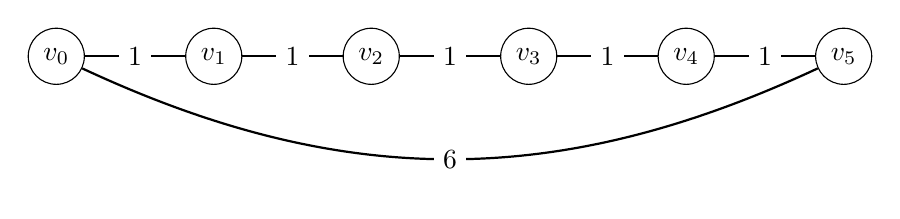
\begin{tikzpicture}[round/.style={circle, draw=black, thin, minimum size=.5mm}, transform shape, scale=1]
    \node[round](0) at (0,0){$v_{0}$};
    \node[round](1) at (2,0){$v_{1}$};
    \node[round](2) at (4,0){$v_{2}$};
    \node[round](3) at (6,0){$v_{3}$};
    \node[round](4) at (8,0){$v_{4}$};
    \node[round](5) at (10,0){$v_{5}$};

    \Edge[label=$1$](0)(1)
    \Edge[label=$1$](1)(2)
    \Edge[label=$1$](2)(3)
    \Edge[label=$1$](3)(4)
    \Edge[label=$1$](4)(5)

    \tikzset{EdgeStyle/.style={bend right=25}} %Arestes m�ltiples
    \Edge[label=$6$](0)(5)
    \end{tikzpicture}
\end{figure}
\end{frame}

\begin{frame}[fragile]
\frametitle{Exemple d'execuci�}
\begin{minted}[breaklines=true, frame=lines, fontsize=\footnotesize]{python}
metro(metro_barcelona, "4_Llucmajor", "9S_Aeroport T1", 25)
\end{minted}
\begin{minted}[breaklines=true, frame=lines, fontsize=\footnotesize]{text}
Punt inicial: 4_Llucmajor
Punt final: 9S_Aeroport T1
Temps net del recorregut: 3565
Temps total del recorregut: 59 minuts i 25 segons
Recorregut: [ 4_Llucmajor, 4_Maragall, 4_Guinard� Hospital de Sant Pau, 4_Alfons X, 4_Joanic, 4_Verdaguer, 5_Verdaguer, 5_Diagonal, 5_Hospital Cl�nic, 5_Enten�a, 5_Sants Estaci�, 5_Pla�a de Sants, 5_Badal, 5_Collblanc, 9S_Collblanc, 9S_Torrassa, 9S_Can Tries Gornal, 9S_Europa Fira, 9S_Fira, 9S_Parc Log�stic, 9S_Mercabarna, 9S_Les Moreres, 9S_El Prat Estaci�, 9S_C�ntric, 9S_Parc Nou, 9S_Mas Blau, 9S_Aeroport T2, 9S_Aeroport T1 ]
\end{minted}
\end{frame}

\section{Conclusions}
\begin{frame}
\frametitle{Conclusions}
\begin{itemize}
\item Objectius assolits.
\item Podem trobar grafs a una gran quantitat d'�mbits i amb moltes aplicacions diferents.
\item Import�ncia de la computaci� en procediments matem�tics.
\item Queda molta feina per fer.
\end{itemize}
\end{frame}

\begin{frame}
\frametitle{Programari lliure}
\begin{itemize}
\item Ubuntu i Debian com a S.O.
\item Python com a llenguatge de programaci�
\item LaTeX i els seus paquets per a la redacci� de la mem�ria
\item Git com a sistema de control de versions
\item Geogebra, Spyder, Scilab, Vim, Meld... i molts d'altres!
\end{itemize}
\end{frame}


\begin{frame}
\centering
M�s informaci� del treball a\\
\Large{\textbf{aniolgarcia.github.io/grafs}}\\
\vspace{1cm}

\Huge{\textbf{Moltes gr�cies!}}\\
\vspace{1cm}

\large{\textbf{Aniol Garcia i Serrano}}\\
aniolgarcia@gmail.com

\end{frame}

\end{document}
